% !TeX encoding = UTF-8
% !TeX spellcheck = en_US
% !TeX root = ../../Thesis.tex

\chapter{CRT handling}
\label{chap:CRT handling}

\section{Opening CRTs}
\label{sec:Opening CRTs}

In order to use hit the $^{39}\mathrm{K}$ cloud with an electron beam, it is necessary to cut open the CRT. This section explains the different methods which were tried and which resulted in clean and easy cuts. All slices were made in a glove box filled with nitrogen gas (\cref{fig:glovebox}) to avoid oxygen poisoning of the cathode.

\begin{figure}[h]
	\missingfigure[figwidth=0.9\textwidth]{Image of glove box.}
	
	\caption{Glovebox filled with nitrogen gas to open CRTs.}
	\label{fig:glovebox}
\end{figure}


\subsection{Rotary tool}
\label{subsec:Rotary tool}


First, a small hole was drilled in the center of the CRT pins to pressurize the CRT with nitrogen. Then a diamond wheel attached to a rotary tool \todo[caption={Dremel trademark}]{\href{https://en.wikipedia.org/wiki/List_of_generic_and_genericized_trademarks}{link}} was used to cut the glass. This method was tried twice, but did not work well the second time. (\todo{Ask Thomas} Why did it not work well? Did the diamond wheel break?) Another obstacle is the plastic box, since it is not fully transparent and therefore made more difficult to see inside. Furthermore, glass dust adhered on the plastic and made it even harder to see the CRT from outside.


\subsection{Wire cutting}
\label{subsec:Wire cutting}

Higher success was achieved by cutting the glass with a heated wire. Two wires were put through the glove box with each inside ending being a ring terminal. A small height adjustable gadget was built out of optical table parts (\cref{fig:Gadget to cut CRT with wire}) in which the CRT was put vertically and looped by a thin wire \todo{wire dimensions, material}. When looping the wire it is important to keep a small gap to avoid an electrical short. Therefore two notches were made in which the wire was fixed.

The assembly was put inside the glove box which was subsequently filled with nitrogen. A current of approximately \SIrange{2}{2.5}{\ampere} was used to heat the thin wire which will result in a breaking point inside the CRT glass. This method does not require a CRT pressurization before the cut. In order to not destroy a device by mistake, this procedure can be first tested on drinking glasses.

\begin{figure}[h]
	\missingfigure[figwidth=0.9\textwidth]{Image of gadget.}
	
	\caption{Gadget to cut CRT with wire.}
	\label{fig:Gadget to cut CRT with wire}
\end{figure}


\section{Oxygen poisoning}
\label{sec:Oxygen poisoning}


As mentioned in \todo{where ?} it is paramount to avoid contact of the cathode with oxygen. Therefore tests with a broken CRT were made to test on how well it can be isolated from air.

% daily notes 2019-12-11
The first experiment consisted of filling a drinking glass put upside-down with helium and putting a lighter after a set amount of time. If the fire goes off, it means that oxygen did not get inside. This was tested successfully from \SIrange{0.5}{10}{\minute}.

Next, plastic wrap was put on top of the glass filled with nitrogen by a rubber band. The glass was put with the open side up from \SIrange{3}{10}{\minute} after which it was turned upside down and the foil was removed. A lighter was put inside and the flame went out again.

To improve the sensitivity, a He leak tester was used. For the first two tests, one plastic foil and one rubber band were used, for the third test three foils and two rubber bands, and for the last test an aluminum foil was hot glued on the CRT to seal it. The measurement locations are shown in \cref{fig:Measurement locatiosn of He leakage}. As shown in \cref{tab:He leak test series.} \todo{which table better?} using rubber band and clear foil results in the highest leakage while the glue seals much better (glue avg). But care needs to be taken in order ensure that the whole CRT is sealed since even a small leak can result in a rate around an order of magnitude above the background (glue max).

\begin{table}[h]
	\centering
	\caption{He leak test.}
	\label{tab:He leak test series.}
	
	\begin{tabular}{l S}
		\toprule
		
		location & {leak rate/(\si{\milli\bar\litre/\second})} \\
		\midrule
		
		% 1st video
		\multicolumn{2}{l}{1 plastic foil, 1 rubber band} \\
		background & \num{8e-5} \\
		plastic foil & \num{2e-4} \\
		He gas cylinder & \num{2e-3} \\
		\midrule
		
		% 2nd video
		\multicolumn{2}{l}{1 plastic foil, 1 rubber band} \\
		background & \num{7e-5} \\
		plastic foil & \num{2e-4} \\
		rubber band & \num{4e-4} \\
		\midrule
		
		% 3rd video
		\multicolumn{2}{l}{3 foils, 2 rubber bands} \\
		background & \num{2e-4} \\
		plastic foil & \num{3e-4} \\
		rubber band & \num{7e-4} \\
		\midrule
		
		% 4th video
		\multicolumn{2}{l}{1 aluminum foil, hot glue} \\
		background & \num{6e-5} \\
		glue avg & \num{7e-5} \\
		glue max & \num{6e-4} \\
		aluminum foil & \num{8e-5} \\
		\bottomrule
	\end{tabular}
\end{table}

\begin{table}[h]
	\centering
	\caption{He leak test.}
	%\label{tab:He leak test series.}
	\todo[inline]{numbers right aligned}
	
	\begin{tabular}{l S}
		\toprule
		
		location & {leak rate/(\SI{e-5}{\milli\bar\litre/\second})} \\
		\midrule
		
		% 1st video
		\multicolumn{2}{l}{1 plastic foil, 1 rubber band} \\
		background & \num{8} \\
		plastic foil & \num{20} \\
		He gas cylinder & \num{200} \\
		\midrule
		
		% 2nd video
		\multicolumn{2}{l}{1 plastic foil, 1 rubber band} \\
		background & \num{7} \\
		plastic foil & \num{20} \\
		rubber band & \num{40} \\
		\midrule
		
		% 3rd video
		\multicolumn{2}{l}{3 foils, 2 rubber bands} \\
		background & \num{20} \\
		plastic foil & \num{30} \\
		rubber band & \num{70} \\
		\midrule
		
		% 4th video
		\multicolumn{2}{l}{1 aluminum foil, hot glue} \\
		background & \num{6} \\
		glue min & \num{7} \\
		glue max & \num{60} \\
		aluminum foil & \num{8} \\
		\bottomrule
	\end{tabular}
\end{table}

\begin{figure}[h]
	\centering
	
	\begin{subfigure}[b]{0.4\textwidth}
		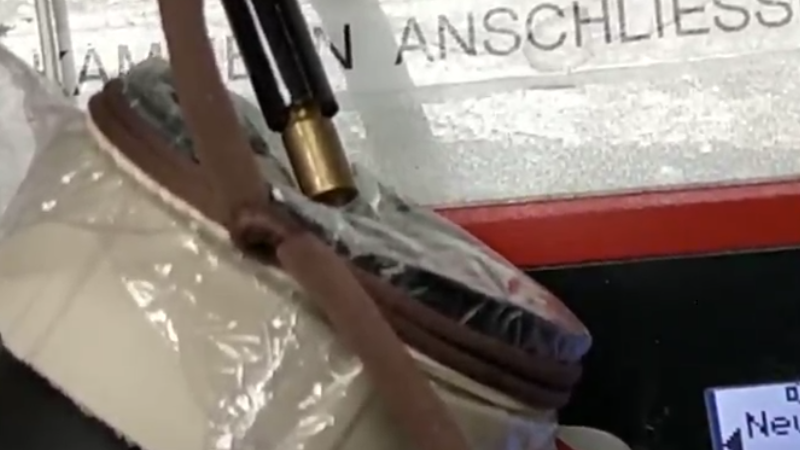
\includegraphics[width=\textwidth]{./Chapters/CRT-handling/plastic_foil}
		\caption{plastic foil}
	\end{subfigure}
	\hspace{0.1\textwidth}
	\begin{subfigure}[b]{0.4\textwidth}
		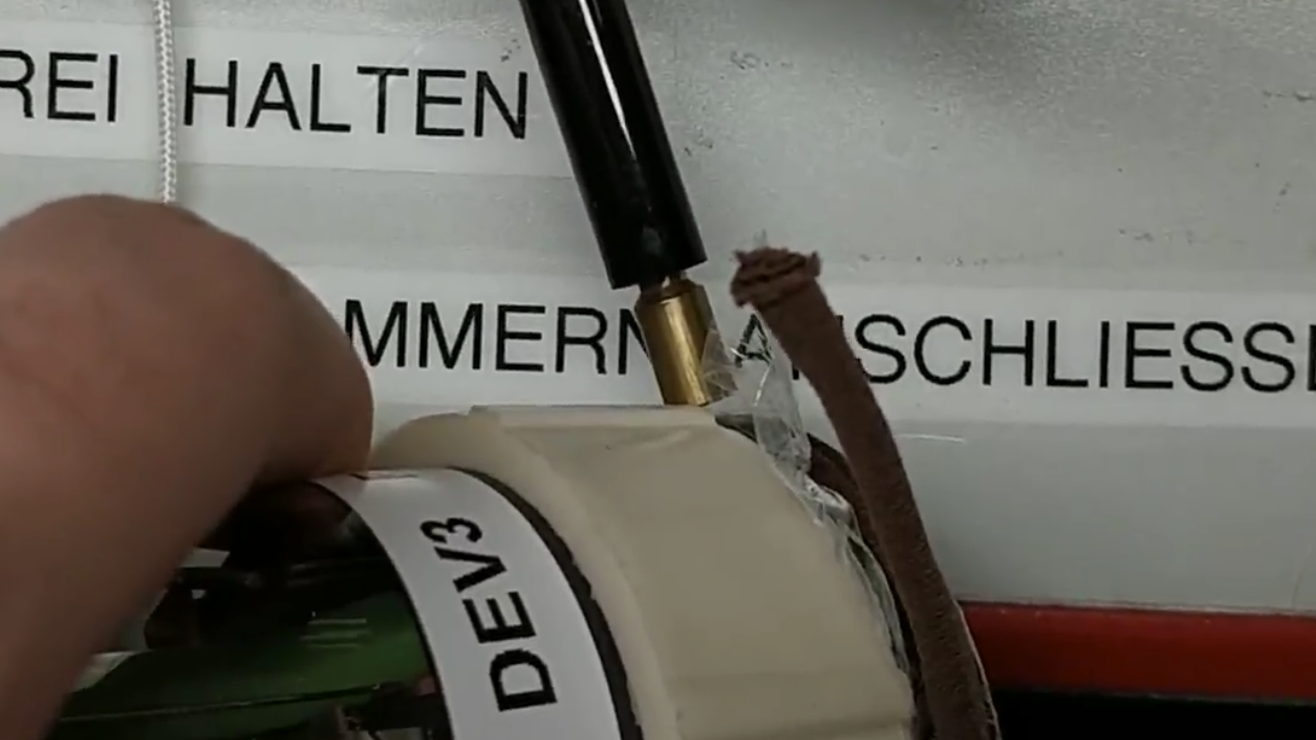
\includegraphics[width=\textwidth]{./Chapters/CRT-handling/rubber_band}
		\caption{rubber band}
	\end{subfigure}

	\vspace{1cm}
	
	\begin{subfigure}[b]{0.4\textwidth}
		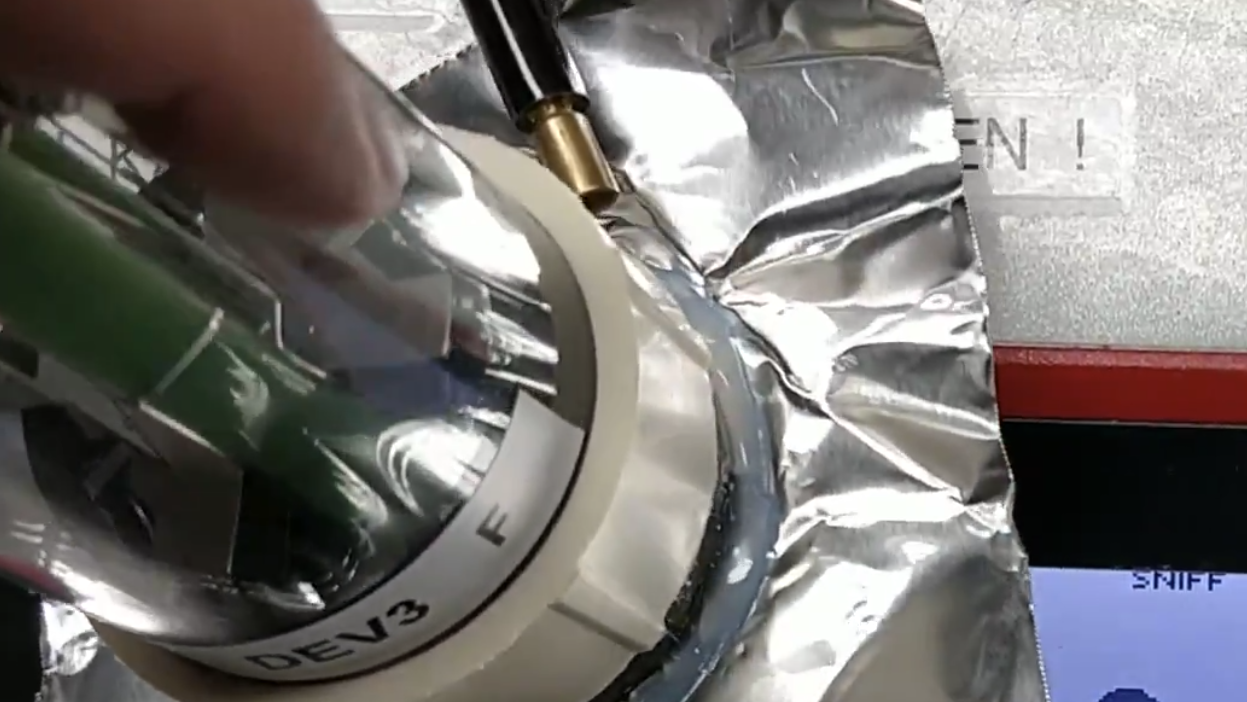
\includegraphics[width=\textwidth]{./Chapters/CRT-handling/glue}
		\caption{glue}
	\end{subfigure}
	\hspace{0.1\textwidth}
	\begin{subfigure}[b]{0.4\textwidth}
		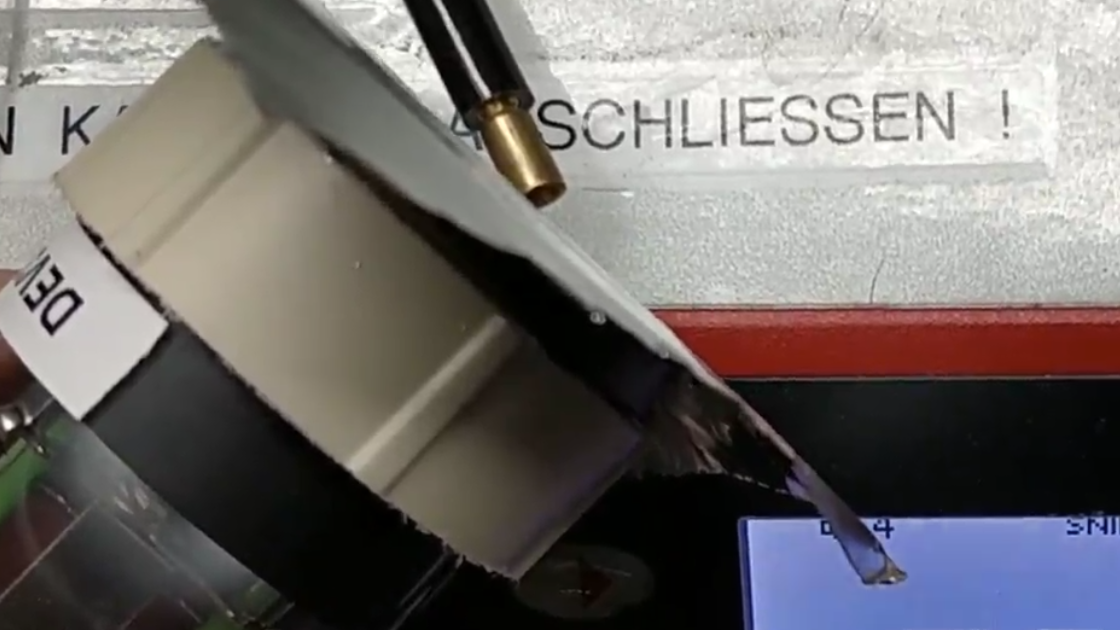
\includegraphics[width=\textwidth]{./Chapters/CRT-handling/aluminum_foil}
		\caption{aluminum}
	\end{subfigure}
	
	\caption{Measurement locations of He leakage.}
	\label{fig:Measurement locatiosn of He leakage}
\end{figure}
 


